\chapter{Cenni alla Chinesiologia}
%\myChapter{Cenni alla Chinesiologia}
\label{cap:chinesiologia}
$\kappa\iota\nu\eta\sigma\iota\varsigma \quad (kin\bar{e}sis)$:  mobilit�,\\
$\lambda o\gamma \iota \alpha \quad (logia)$: studio di\\

\begin{quotation}
%The study of the principles of mechanics and anatomy in relation to human movement.
Lo studio dei principi su cui si fondano la meccanica e l'anatomia del movimento umano. 
\end{quotation}
\begin{flushright}
\emph{www.merriam-webster.com}\cite{merriam-webste_Online}
\end{flushright}
\vspace{1cm}

La Chinesiologia studia il movimento umano sotto diversi aspetti: biomeccanico, del controllo motorio e della psicologia del moto.\\
L'approccio biomeccanico \cite{Hall_basic_biomechanics} consiste nell'applicazione dei principi della Meccanica allo studio di organismi viventi: principalmente propriet� fisiche di materiali biologici, segnali biologici, modellazioni e simulazioni biomeccaniche.

Per restringere l'ambito, noi ci concentriamo sulle interazioni biomeccaniche dell'apparato locomotore (scheletro e muscoli).
La branca della Meccanica Classica (vedi appendice \ref{meccanica_classica}) 
che viene utilizzata dalla Biomeccanica � la Cinematica \cite{Encyclopedia_Britannica_online}
che si occupa di descrivere la posizione ed il moto di oggetti nello spazio, senza riferimento alle forze o masse coinvolte (vale a dire alle cause e agli effetti di tale moto). 

\section{Analisi dei movimenti del corpo umano}
Per un trattamento rigoroso dei movimenti del corpo umano, � necessario stabilire dei piani di riferimento, lungo i quali collocare le diverse parti del corpo (vedi figura \ref{fig:HumanBodySPL}).

\begin{figure}
	\centering
		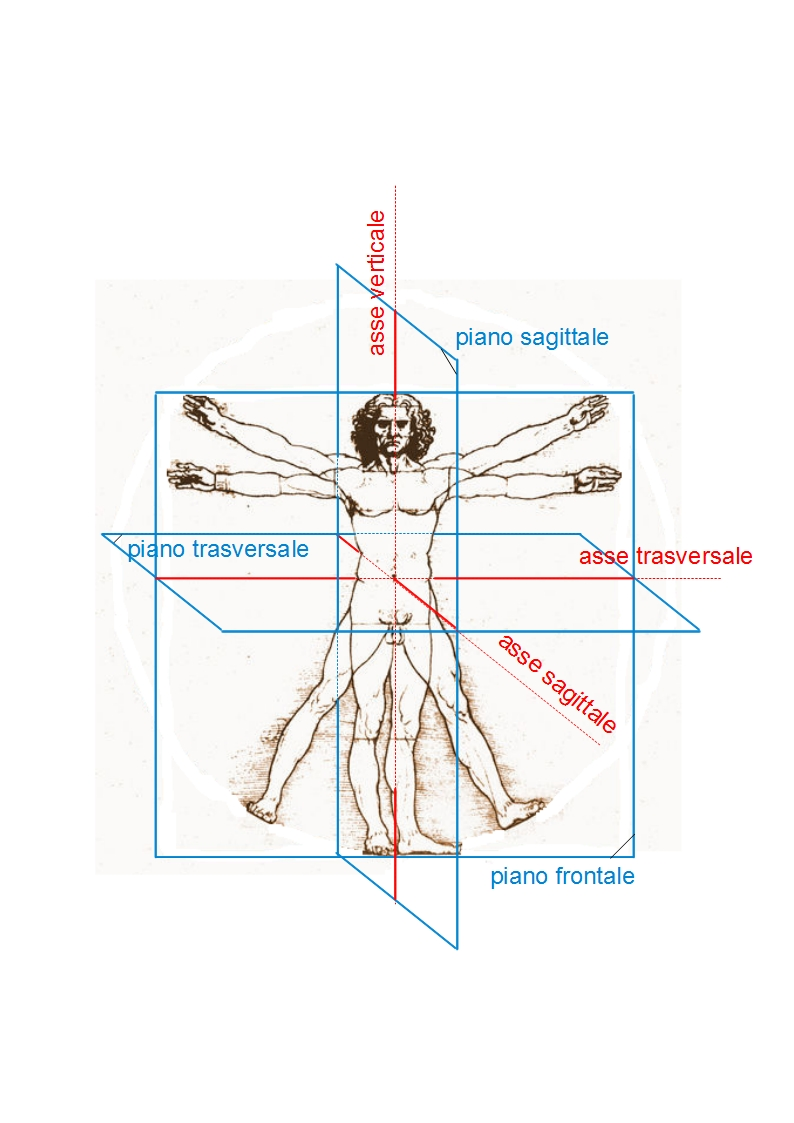
\includegraphics[width=0.90\textwidth]{imgs/Human_body_by_Da_Vinci-SPL.jpg}
	\caption{Immagine riadattata. Originale cortesia di \url{http://sciencephoto.com} }
	\label{fig:HumanBodySPL}
\end{figure}

\begin{definition}[Piani che tagliano il corpo umano]
I movimenti del corpo umano vengono descritti in riferimento a tre piani:
	\begin{enumerate}
		\item \textbf{Frontale o Coronale}:  piano verticale che divide il corpo in parte anteriore e posteriore.
		\item \textbf{Sagittale}: piano verticale che divide il corpo in parte sinistra e destra.
		\item \textbf{Trasversale o Orizzontale}: piano orizzontale che divide il corpo in parte superiore ed inferiore. 
	\end{enumerate}
\end{definition}
Ad esempio la deambulazione o corsa avviene principalmente lungo il piano sagittale, sollevare le braccia lateralmente comporta un movimento sul piano frontale, mentre la rotazione della testa per guardarsi intorno avviene principalmente lungo il piano trasversale. 


\section{L'andatura durante la deambulazione}
Viene definita Andatura (Gait) la sequenza di movimenti degli arti inferiori che un animale compie su una superficie solida durante la locomozione \cite{Herbrand_gait}. Gli animali possiedono diverse forme di andatura che scelgono in base alla velocit�, ed al terreno ed ad altre variabili. \\
La Deambulazione (o Camminata) � una delle principali forme di andatura degli animali aventi arti inferiori ed avviene tipicamente a velocit� inferiore a quelle della Corsa (che a sua volta � una forma di locomozione).  
\begin{definition}[Deambulazione Normale]
\label{deambulazione_normale}
Una Deambulazione normale (negli esseri umani) � composta di due macro fasi per ciascun piede: 
\begin{enumerate}
	\item fase di appoggio (Stance), in cui il piede supporta tutto il peso del corpo e
	\item Fase in aria (Swing), in cui il piede � in aria e porta avanti il baricentro del corpo, mentre il peso del corpo � sull'altro piede.
\end{enumerate}
I due arti inferiori sono sempre alternativamente nelle due fasi e per circa il 25\% del tempo sono in contatto simultaneo con il pavimento.
\end{definition}


\section{Breve storia dello studio della deambulazione umana}
Un primissimo contributo allo studio dell'andatura umana � stato dato dai  fratelli Wilhelm Weber, fisico, e Eduard Weber, anatomista. I Weber, nel loro libro \emph{The Mechanics of Human Motions} \cite{Weber_mechanics_human_motion}, pubblicato nel 1836, definiscono e misurano per la prima volta la durata delle fasi della Deambulazione Normale (vedi definizione \ref{deambulazione_normale}), usando solamente un cronometro ed un telescopio con una scala.\\
Un grande contributo a questo campo � stato dato dal fisiologo francese $\grave{E}$tienne Jules Marey, che nel 1873 pubblic� il trattato  \emph{Animal Mechanism: a Treatise on Terrestrial and Aerial Locomotion} dove con l'uso di scarpe a camera d'aria collegate a un registratore e della {Cronofotografia Geometrica}\footnote{pi� riprese fotografiche vengono impresse sulla stessa fotografia, in modo che possa essere ripresa una sequenza di azioni della persona. Si tratta di un antenato della cinepresa.} e con l'uso di soggetti vestiti con abiti aderenti e neri con bottoni di metallo e strisce riflettenti, riusci� a misurare la durata del contatto del piede con il suolo, durante la camminata in piano, su un terreno regolare. Inoltre egli introdusse il concetto dell'efficienza energetica del movimento.\\
Il fotografo inglese Edward Muybridge, nel 1887 con l'uso della fotografia seriale, con 48 fotocamere elettriche sincronizzate riusci� a catturare la fase in volo di un cavallo al galoppo.\\
L'anatomista tedesco Wilhelm Braune, ed il matematico tedesco Otto Fisher, negli anni 1890, con l'uso di un sistema a 4 fotocamere, un tubo luminoso attaccato al corpo ripreso ed un sistema di riferimento rettangolare, riuscirono a analizzare per la prima volta l'andatura in 3D ed a stabilire i metodo per il calcolo dei parametri meccanici dello stesso. \\
Nel 1938 Elftman e 20 anni dopo Frankel diedero grossi contributi agli studi di tipo cinetico sul {passo normale e patologico}\footnote{passo affetto da una qualunque tipo di deformazione rispetto al passo normale}.\\
M.P. Murray, negli anni '60, con l'uso della fotografia a luce interrotta e pi� tardi con il sistema 3D, diede dei contributi allo studio cinetico in pazienti normali e patologici. \\
J Perry con l'uso di goniometri elettronici monoassiali ha sviluppato un nuovo sistema di terminologie per l'andatura sia normale che patologica. 

\section{Ciclo di deambulazione (Gait Cycle)}
L'unit� di base per la descrizione dell'andatura nella deambulazione � il ciclo di andatura (Gait Cycle) (vedi figura \ref{fig:CicoloDelPasso}). Si tratta della sequenza di azioni compiute dal corpo dall'istante dell'impatto di un tallone a terra fino al impatto successivo dello stesso tallone. Il ciclo di andatura ha una durata compresa nell'intervallo di [0.5-2] secondi, in base alla velocit�. Il ciclo di andatura � suddiviso in due fasi: una di appoggio, in cui il piede � a contatto con il terreno, ed una aerea. 
\begin{figure}[h]
	\centering
		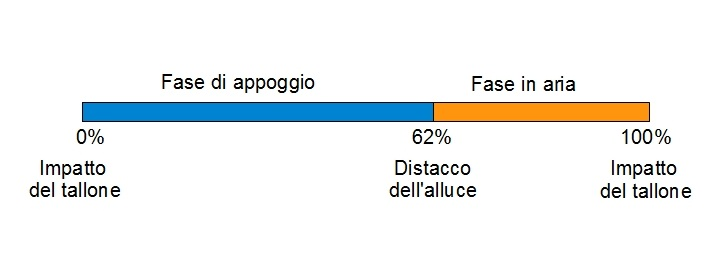
\includegraphics[width=0.95\textwidth]{imgs/CicoloDelPasso.jpg}
	\caption{Ciclo completo di andatura }
	\label{fig:CicoloDelPasso}
\end{figure}

%La fase di appoggio (dal contatto del tallone al distacco dell'alluce dal terreno) viene ulteriormente suddivisa in tre sottofasi: 
%\begin{enumerate}
%	\item contatto iniziale;
%	\item appoggio intermedio (detta anche fase di risposta al carico);
%	\item fase propulsiva (o di contatto finale).
%\end{enumerate}
 

%\section{Gait Cycle}
\begin{figure}[h]
	\centering
		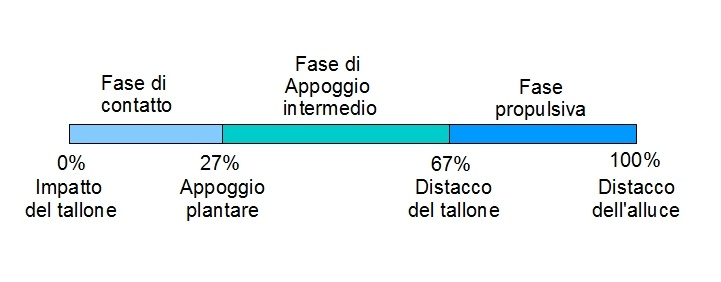
\includegraphics[width=0.95\textwidth]{imgs/CicoloDelPassoAppoggio.jpg}
	\caption{Fase di appoggio}
	\label{fig:CicoloDelPassoAppoggio}
\end{figure}


Le due fasi possono essere ulteriormente suddivise. In queste vi sono eventi che determinano l'inizio e la fine di una fase. Per definizione un ciclo di deambulazione inizia e termina con la fase HS (Heel Strike) ovvero impatto del tallone con il suolo. All'evento HS cui segue la fase LR (Load Response) fase di risposta al carico, ovvero il peso del corpo si sposta per gran parte sul piede avanti. A termine della fase LR, si verifica l'evento FF (Foot Flat) appoggio plantare, in cui il piede avanti si trova piatto sul suolo. L'evento FF � seguito dalla fase MS (Mid Stance) fase di appoggio intermedio in cui il corpo si propelle in avanti ed il piede indietro si innalza da. L'evento che termina la fase MS � HO (Heel Off) distacco del tallone, che indica la transizione ad una transizione tra la fase TS (Terminal Stance) propulsione ed una breve fase nota come PSw (Pre Swing) pre distacco che precede la fase in aria. In questa transizione il corpo viene nuovamente spinto in avanti, e tale spinta provoca l'ultimo evento della fase di appoggio del piede ovvero TO (Toe Off) distacco dell'alluce. Dopo TO inizia la fase in aria del piede. In questa fase il piede in aria si porta davanti al piede portante permettendo cos� l'inizio di un nuovo ciclo di deambulazione. Anche la fase in aria pu� essere suddivisa in tre sottofasi: ISw (Initial Swing) propulsione iniziale in cui l'arto viene accelerato, MSw (Mid Swing) propulsione mediale in cui l'arto per aria sorpassa quello a terra ed infine TSw (Terminal Swing) decelerazione, in preparazione per l'atterraggio, ovvero l'evento iniziale HS. 
 

\begin{table}%
\begin{tabular}{|m{5cm}|m{5cm}|m{.5cm}}
\cline{1-2}
\textsc{Evento} & \textsc{Fase}&\\
\cline{1-2}
\cline{1-2}
\textbf{HS} - impatto del tallone&&\\
\cline{2-2}
& LR - risposta al carico&\multirow{6}{*}{\rotatebox{90}{Fase di appoggio}}\\
\cline{2-2}
\textbf{FF} - appoggio plantare &&\\
\cline{2-2}
& MS - appoggio intermedio&\\
\cline{2-2}
\textbf{HO} - distacco del tallone &&\\
\cline{2-2}
& TS - propulsione&\\
\cline{2-2}
& Psw - pre distacco&\\
\cline{2-2}
\textbf{TO} - distacco dell'alluce &&\\
\cline{1-2}
& ISw - accelerazione&\multirow{3}{*}{\rotatebox{90}{Fase in aria}}\\
\cline{2-2}
& MSw - superamento&\\
\cline{2-2}
& TSw - decelerazione&\\
\cline{2-2}
\textbf{HS}&&\\
\cline{1-2}
\end{tabular}
\newline
\caption{Ulteriori suddivisioni del cammino in eventi e fasi.}
\label{fasi_del_cammino}
\end{table}




\subsection{Confronto fra Falcata (Stride) e Passo (Step)}

La falcata, che va dal impatto del tallone con il suolo fino al successivo contatto dello stesso piede, � sinonimo di ciclo di andatura (Gait Cycle), mentre il passo comincia dal impatto di un tallone e termina al impatto dell'altro tallone. Una falcata coincide esattamente con due passi (vedi figura \ref{fig:AndaturaConfrontoPasso}).
\begin{figure}[h]
	\centering
		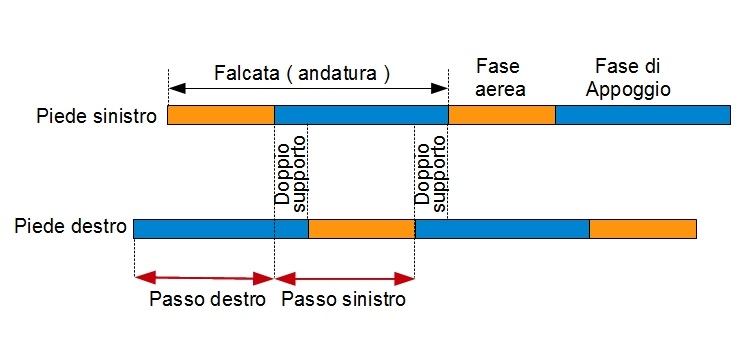
\includegraphics[width=0.95\textwidth]{imgs/AndaturaConfrontoPasso.jpg}
	\caption{Andatura e Passo a confronto}
	\label{fig:AndaturaConfrontoPasso}
\end{figure}

\section{Parametri che descrivono il pattern (schema) della deambulazione}
%\begin{wraptable}{r}[-9mm]{0.30\textwidth}
\begin{table}%
\begin{tabular}{|p{3cm}|p{2cm}|p{5cm}|}
\hline
\textsc{nome parametro} & \textsc{unit� di misura} & \textsc{descrizione}\\
\hline
\hline
Andatura &(sec)& durata di un completo ciclo di andatura\\
\hline
Passo &(sec)& durata di un completo passo sinistro o destro\\
\hline
Contatto &(sec, \%)& durata del periodo in cui i piedi rimangono a contatto con il terreno\\
\hline
Contatto a piede singolo &(sec, \%)&durata del periodo in cui solo un piede rimane a contatto con il terreno\\
\hline
Doppio contatto &(sec, \%)& durata del periodo in cui entrambi piede rimangono contemporaneamente a contatto con il terreno\\
\hline
Fase aerea &(sec, \%)& durata del perodo in cui il piede � in aria\\
\hline
\end{tabular}
\newline
\caption{Parametri temporali}
\label{parametri_temporali}
\end{table}
%\end{wraptable}


\begin{table}%
\begin{tabular}{|p{3cm}|p{2cm}|p{5cm}|}
\hline
\textsc{nome parametro} & \textsc{unit� di misura} & \textsc{descrizione}\\
\hline
\hline
Lunghezza dell'andatura &(cm)& distanza tra due punti di impatto successivi dello stesso tallone\\
\hline
Lunghezza del passo &(cm)& distanza tra due punti di impatto successivi di talloni opposti\\
\hline
Larghezza del passo &(cm)&distanza laterale tra due punti di impatto successivi di talloni opposti\\
\hline
Angolo del piede &(grad)& angolo tra il collo del piede e lo stinco \\
\hline
\end{tabular}
\newline
\caption{Parametri spaziali}
\label{parametri_spaziali}
\end{table}


\begin{table}%
\begin{tabular}{|p{3cm}|p{2cm}|p{5cm}|}
\hline
\textsc{nome parametro} & \textsc{unit� di misura} & \textsc{descrizione}\\
\hline
\hline
Cadenza & (passi/ min) & numero di passi al minuto\\
\hline
Velocit� del passo &(m/s) & numero di metri percorso al secondo \\
\hline
\end{tabular}
\caption{Parametri di velocit�}
\label{parametri_velocit�}
\end{table}